% imports
\documentclass[12pt, a4paper]{article}
\usepackage{mathptmx} % FONT
\usepackage{fancyhdr}
\usepackage[utf8]{inputenc}
\usepackage{graphicx}
\usepackage[margin = 0.6in, includeheadfoot]{geometry}
\usepackage{float}
\usepackage{amsmath}
\usepackage{hyphenat}
\usepackage{tikz}
\usepackage{pgfplots}
\usepackage[]{minted}
\usepackage[fancyvrb=true]{listings}
\usepackage{etoolbox}
\usepackage{csquotes}
\usepackage{tcolorbox}
\usepackage[title, titletoc]{appendix}
\usepackage{float}
\usepackage{titlesec}
\usepackage{multirow}
\usepackage{multicol}
\usepackage{array}
\usepackage{url}
\usepackage[hidelinks]{hyperref}
\usepackage{siunitx}
\usepackage{circuitikz}
\usepackage{tikz-timing}
\usepackage{physics}
\usepackage{setspace}
\usepackage{svg}
\usepackage{epsfig}
\usepackage{titlesec}
\titleformat{\paragraph}[hang]{\normalfont\normalsize\bfseries}{\theparagraph}{1em}{}
\titlespacing*{\paragraph}{0pt}{3.25ex plus 1ex minus .2ex}{1em}
\onehalfspacing
\setcounter{tocdepth}{3}
\setcounter{secnumdepth}{5}





%styling
\usemintedstyle{vs}
\BeforeBeginEnvironment{minted}{\begin{tcolorbox}}
\newminted{vhdl}{frame=lines, framerule=1pt}
\AfterEndEnvironment{minted}{\end{tcolorbox}}
\setlength{\headheight}{14.88316pt}
\pagestyle{fancy}
\topmargin = -35pt
\setlength{\parskip}{0.5em}
\setlength{\parindent}{0em}
\fancyhf{} % Clear all header and footer fields
\fancyhead[L]{\textit{\nouppercase{\leftmark}}} % Left header: section name
\fancyhead[R]{\thepage} % Right header: page number
\renewcommand{\headrulewidth}{0.4pt} % Line below the header

\usepackage{listings}
\usepackage{color} %red, green, blue, yellow, cyan, magenta, black, white
\definecolor{mygreen}{RGB}{28,172,0} % color values Red, Green, Blue
\definecolor{mylilas}{RGB}{170,55,241}


% Default fixed font does not support bold face
\DeclareFixedFont{\ttb}{T1}{txtt}{bx}{n}{12} % for bold
\DeclareFixedFont{\ttm}{T1}{txtt}{m}{n}{12}  % for normal

% Custom colors
\usepackage{color}
\definecolor{deepblue}{rgb}{0,0,0.5}
\definecolor{deepred}{rgb}{0.6,0,0}
\definecolor{deepgreen}{rgb}{0,0.5,0}

\usepackage{listings}

% Python style for highlighting
\newcommand\pythonstyle{\lstset{
language=Python,
basicstyle=\ttm,
morekeywords={self},              % Add keywords here
keywordstyle=\ttb\color{deepblue},
emph={MyClass,__init__},          % Custom highlighting
emphstyle=\ttb\color{deepred},    % Custom highlighting style
stringstyle=\color{deepgreen},
frame=tb,                         % Any extra options here
showstringspaces=false
}}


% Python environment
\lstnewenvironment{python}[1][]
{
\pythonstyle
\lstset{#1}
}
{}

% Python for external files
\newcommand\pythonexternal[2][]{{
\pythonstyle
\lstinputlisting[#1]{#2}}}

% Python for inline
\newcommand\pythoninline[1]{{\pythonstyle\lstinline!#1!}}


\begin{document}






\begin{titlepage}
     \begin{tikzpicture}[remember picture, overlay]
    \node[anchor=north, inner sep = 0pt] at (current page.north)
        {
\includegraphics[scale=1.1]{IMAGES/strath logo.jpg}};
    \end{tikzpicture}
     \centering
    
    \vspace{5cm}
    {\normalsize \enquote{I hereby declare that this work has not been submitted for any other degree/course at this University or any other institution and that, except where reference is made to the work of other authors, the material presented is original and entirely the result of my own work at the University of Strathclyde under the supervision of Dr Louise H Crockett.}}

    \vspace{5cm}
    {\huge\bfseries SDR Application Using GNU Radio on RFSoC Platform\par}
    {\huge Fraser O'Regan 202115033\par}
    \vspace{1cm}
    {\Large Supervisor: Dr Louise H Crockett\par}
    {\Large April 2025\par}
    \vfill
\end{titlepage}
\section*{Acknowledgements}



\newpage
\tableofcontents
\newpage



\section*{Nomenclature}
\begin{itemize}
    \item \textcolor{red}{\large Fix references to all have same format and include access dates}
    \textcolor{red}{GO THROUGH AND FIX NOMENCLATURE and equation symbols}
\end{itemize}
\addcontentsline{toc}{section}{Nomenclature}


\subsection*{Abbreviations}
\begin{tabular}{@{}>{$}l<{$} l} % Math mode in the first column
\textbf{DSP} & Digital Signal Processing \\
AI & Artificial Intelligence \\
SDR & Software-Defined Radio \\
RF & Radio Frequency \\
GUI & Graphical User Interface\\
SoC & System-on-chip\\
IC & Integrated Circuit\\
PS & Processing System\\
PL & Programmable Logic\\
FPGA & Field Programmable Gate Array\\
SD-FEC & Soft Decision Forward Error Correction\\
RFDC & Radio Frequency Data Converter\\
DAC & Digital to Analogue Converter\\
ADC & Analogue to Digital Converter\\
HDL & Hardware Description Language \\
RTL & Register Transfer Level\\
HLS & High Level Synthesis\\
AXI & Advanced eXtensible Interface\\
SDK & Software Development Kit\\
XSA & Xilinx Support Archive\\
OS & Operating System\\
AM & Amplitude Modulation\\
OFDM & Orthogonal Frequency Division Multiplexing\\
FT & Fourier Transform
NCO & Numerically Controlled Oscillator\\
LUT & Look Up Table\\
ROM & Read Only Memory\\
SFDR & Spurious Free Dynamic Range\\
MUX & Multiplexer\\
FIR & Finite Impulse Response (Filter) \\
IPI & IP Integrator\\
DMA & Direct Memory Access\\
QSFP & Quad Small Form-factor Pluggable\\
Tcl & Tool command language\\
PLL & Phase Locked Loop
\end{tabular}
\newpage
\subsection*{Symbols}
\begin{tabular}{@{}>{$}l<{$} l} % Math mode in the first column
\mu & Step Size \\
N & Depth of LUT in NCO \\
f_{d} & Desired Frequency From NCO \\
f_{s} & Sampling Frequency \\
n & Number of Bits\\
\end{tabular}

\newpage

\section{Abstract}

%Can put this somewhere

\begin{comment}
    \begin{figure}
    \centering
    \includesvg{IMAGES/RFX-Card.svg}
    \caption{Caption}
    \label{fig:enter-label}
\end{figure}
\end{comment}

\newpage
\section{Introduction}


Modern advancements in Digital Signal Processing (DSP), along with Artificial Intelligence (AI), processing power, and much more has culminated in the birth of the Software-Defined Radio (SDR). SDR utilises the flexibility and configurability of an analogue Radio Frequency (RF) front end \cite{collins2018software}, along with the \textit{on-the-go} adaptable nature of software to create a fully programmable and customisable communications system. SDR is traditionally defined as any radio system in which one or more elements is software-defined. Nowadays, radios can be designed almost entirely in software, allowing for even more flexibility with less reliance on bulky hardware. SDR is the backbone of modern development into communication systems by offering more affordable solutions for delving into the world of 5G and beyond. There are many supporting frameworks for SDR development, but GNU Radio stands above the rest as the most complete software for SDR development. GNU Radio is an open source project built primarily in C++ and Python \cite{gnuradio}. GNU Radio also has its own Graphical User Interface (GUI), the GNU Radio companion, an intuitive block diagram modelling tool which aids in the development of these systems without the need to extensively write and debug software. GNU Radio is configurable with a number of low end hardware devices, however, GNU Radio technically possesses the ability to be ported to any custom hardware that the user may need through an ‘out of tree module’. 

The primary aim of this project is to implement an SDR system on a novel piece of hardware, the BittWare RFX-8440L, marking a new endeavour for BittWare, as this sort of technology has not yet been applied to their custom hardware devices. The objectives include exploring the integration of GNU Radio with the BittWare platform, leveraging its high-performance capabilities to develop a functional SDR system, and evaluating its performance against traditional setups. Additionally, a key aim of the project is to gain familiarity with the architecture of the AMD RFSoC, its supporting toolchains, and design flows. This knowledge will lay a solid foundation for progressing toward the design and development of custom SDR systems. Additionally, with a system up and running some extra goals have been set to provide further challenges in validating the systems design. These include the transmission of radio waves over the air, and the potential to receive and transmit some \enquote{real data}, i.e. text, images, audio, etc. Of course, ensuring proper care and licensing issues have been dealt with before engaging in such activities is imperative when working with wireless transmission.

\newpage
\section{Background \& Literature Review}
\subsection{RFSoC Architecture}
This project will focus on the implementation of the aforementioned software and design techniques onto the Zynq UltraScale+ RFSoC (which from now on will just be referred to as the RFSoC) by AMD \cite{amd_zynq_rfsoc}. The RFSoC is an all configurable system-on-chip (SoC) device targeted towards RF applications \cite{RFSoC_Book}. A system-on-chip is an integrated circuit (IC) that features almost all high level functions needed for computation into a single chip, as opposed to the traditional method of having these different components mounted to the motherboard. This allows for a far smaller and more portable package, making it ideal for applications such as communications, mobile devices, and many more. The RFSoCs architecture features two main sections, the Processing System (PS), and the Programmable Logic (PL). The AMD RFSoC utilises the software programmability of processors, in the form of either two or four ARM cores (depending on the generation), along with the hardware programmability of a Field Programmable Gate Array (FPGA). The PL features a number of different \enquote{hardened} blocks, aptly named due to the fact that they have their own dedicated space on the silicon and can not be reconfigured in either software or hardware. The different hardened blocks can be seen below in Figure \ref{fig:RFSoC_overview}.

\begin{figure}[h]
    \centering
    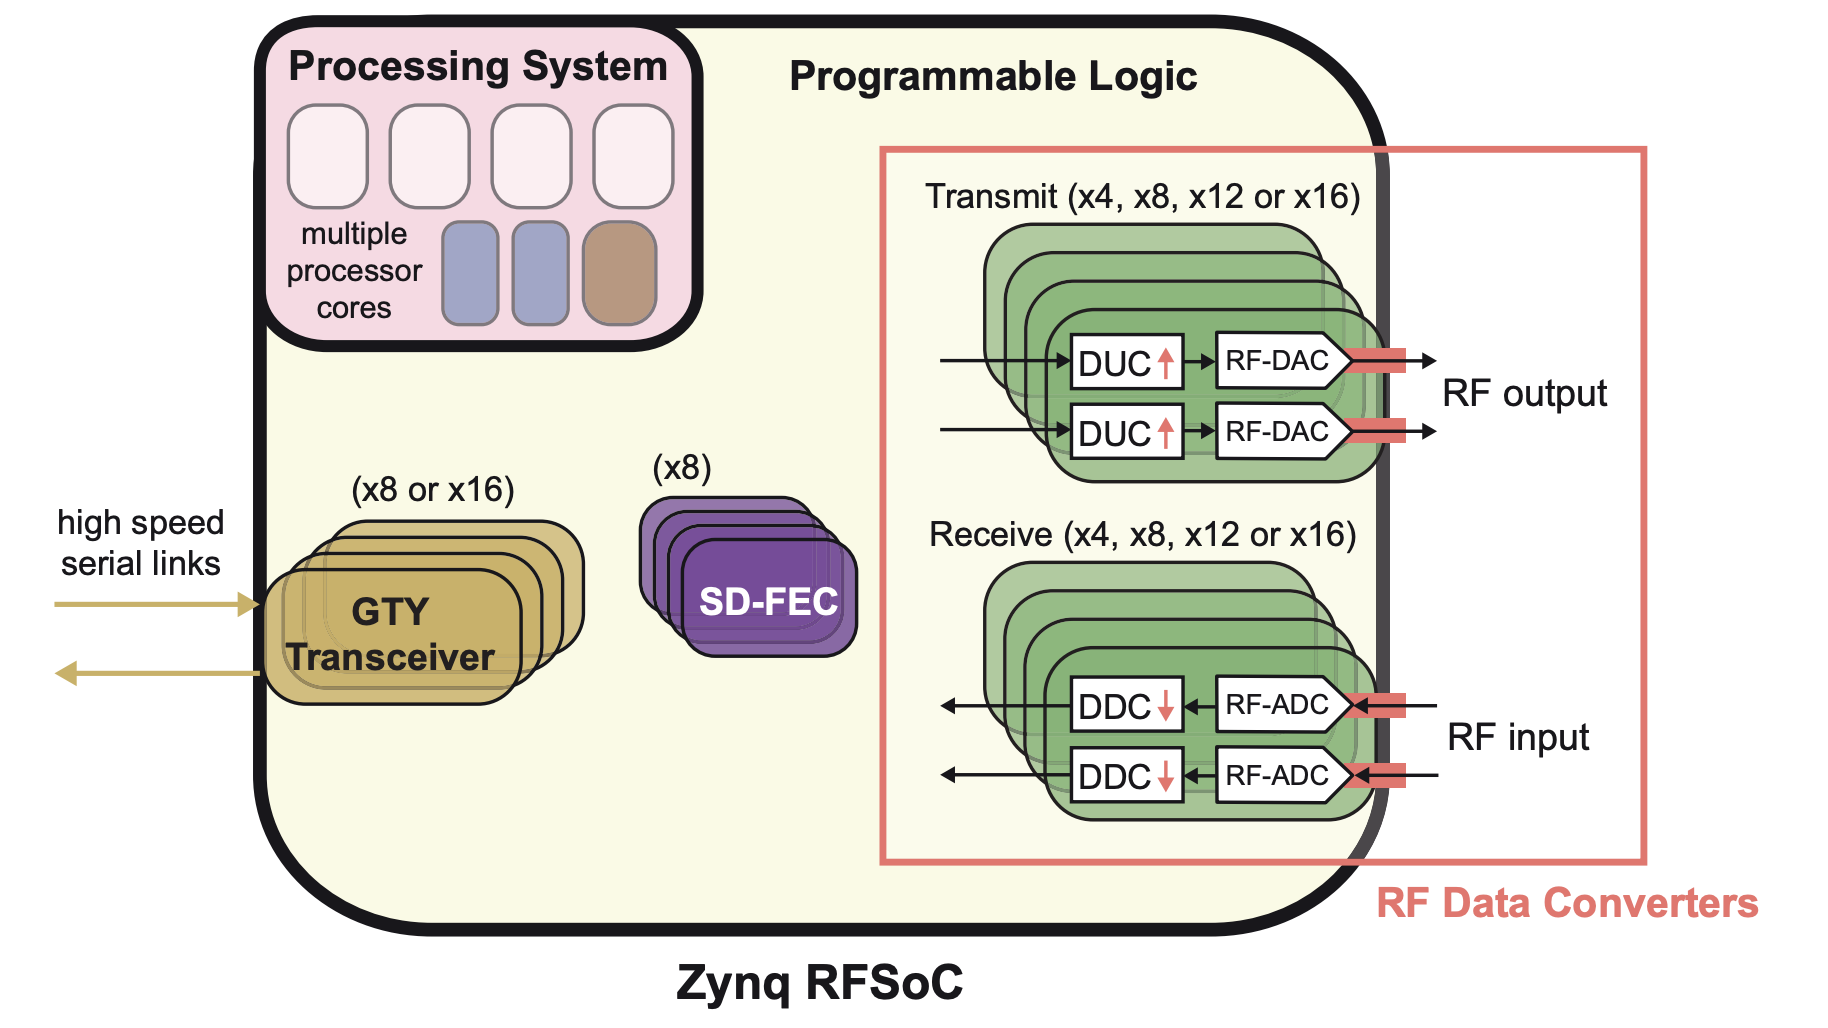
\includegraphics[scale=0.5]{IMAGES/RFSoC_overview_RFSoC_Book.png}
    \caption{High Level Overview of RFSoC Architecture \cite{RFSoC_Book}}
    \label{fig:RFSoC_overview}
\end{figure}

The Advanced eXtensible Interface (AXI) is a communication protocol defined by ARM as part of the Advanced Microcontroller Bus Architecture (AMBA) standard \cite{axi_article}. The AXI4 standard has three different forms: AXI4-Lite, for simple, low-throughput communications,for example, driving an enable register pin; AXI4-Stream, for high-speed streaming data; and full AXI4, which is used for high-performance applications. Typically, embedded systems, such as FPGAs, operate with a master-slave topology between different devices \cite{strathsdr_axi}. The master device can connect to multiple slave devices through a communication protocol, and slave devices can be controlled by multiple masters, executing commands only when driven by a master device. AXI follows this same principle, with read and write channels transferring data between the master and slave components in a hardware design.

AXI4 uses handshake operations, where a handshake is successful when both the valid and ready signals are high on the same clock cycle \cite{strathsdr_axi}. 

\textcolor{red}{need to get photo or graph of axi transactions}

\begin{figure}[h]
    \centering
    \includegraphics[scale=0.2]{}
    \caption{Caption}
    \label{fig:enter-label}
\end{figure}

AXI4-Lite has both a read and write transaction, with the former using the \textbf{read address} and \textbf{read data} channels, and the latter using the \textbf{write address}, \textbf{write data}, and \textbf{write response} channels \cite{strathsdr_axi}. To summarise an AXI4-Lite handshake, the read transaction is performed when the master sends an address on the \textbf{read address} channel, after which the \textbf{valid} and \textbf{ready} signals are asserted, performing the handshake, which is then followed by the read operation where the slave sends the data at the requested memory address using the \textbf{read data} channel. To perform write operations, the master sends an address value using the \textbf{write address} channel, which performs a basic handshake. The master then sends the data that is to be written into the memory address to the slave, this uses the \textbf{write data} channel. Finally, the slave responds using the \textbf{write response} channel, which indicates to the master whether the write operation was successful or not. There is vast support for AXI4-Lite on AMD devices, especially using Model Composer, inputs to designs (Gateway In)(s) can be implemented as an AXI4-Lite register, which allows for simple control once the designs are generated into IP cores in Vivado.
 

AXI4-Stream does not need a memory address channel since it does not move data between different memory locations, but rather moves data between different points on the FPGA. AXI4-Stream uses nine signals, but the most relevant can be seen below in Table \ref{tab:AXI4-Stream signals}.

\begin{table}[h]
    \centering
    \begin{tabular}{|c|c|}\hline
        \textbf{Signal} & \textbf{Function} \\ \hline
         TREADY &  Indicates that the slave device is ready to accept data in the current clock cycle\\ \hline
         TVALID &  Indicates the master is sending valid data. A transfer occurs if TREADY and TVALID are high. \\ \hline
         TDATA & Provides the data that is transferred in an AXI4-Stream transaction \\ \hline
         TLAST & Indicates the last data element in TDATA \\ \hline
    \end{tabular}
    \caption{AXI4-Stream Signal Definitions}
    \label{tab:AXI4-Stream signals}
\end{table}

All AXI4-Stream signals propogate from master to slave, except for TREADY, which travels in the opposite direction. To implement AXI4-Stream in a design, there is a naming convention that must be followed, that is:

\[<Role>\_<ClassName>\_<SignalName>\]

For example, to implement a stream of data on the master side, the signal would be named:

\[m\_\ axis\_\ tdata\]

The AXI4 protocol plays a fundamental role in modern embedded systems, particularly in AMD SoC devices. In this project, AXI4-Stream is essential for efficiently transferring large volumes of data between multiple IP cores within the FPGA, ensuring high-performance communication and system integration.

From left to right, the hardened blocks shown in Figure \ref{fig:RFSoC_overview} are: Gigabit (GTY) transceivers, a high speed serial data link needed for communication to a core network when working with modern communication standards. Additionally, Soft Decision Forward Error Correction (SD-FEC) blocks feature on the chip, since almost all forms of wireless communications require, at some stage, an error correction phase which mitigates against the different errors procured in the wireless channel. Finally, the RFSoC has dedicated RF Data Converter (RFDC) blocks. These blocks can be configured as either Digital to Analogue Converters (DACs), for data transmission, or Analogue to Digital Converters (ADCs), which are used to convert real data to the digital domain, where the signal can be analysed using numerous DSP techniques.

\subsection{Supporting Toolchains and Software}

The PYNQ project by AMD \cite{PYNQ} is another supporting framework that focuses on SoC devices. PYNQ utilises Python application programming interfaces (APIs) to streamline the development of embedded systems on AMD chips. PYNQ itself is a small linux based boot image that runs on the chip, with different commands to control the hardware; however, PYNQ also utilises Jupyter notebooks, in which python code can be ran in different cells, along with accompanying markdown code for readability. Hardware Description Language (HDL) \enquote{bitstreams} can be accessed in the notebook as \enquote{overlays}. The overlays must be used in the project by exporting the Vivado block design, and locating the \textbf{\textit{.hwh}} and \textbf{\textit{.bit}} files. From there, they can be implemented, however an engineer may need and can be reused indefinitely, unless the overlay itself needs to be altered. There are many methods to design a custom overlay to be used in PYNQ; however, the most common ways include writing custom Register Transfer Level (RTL) code using VHDL or Verilog; Writing C/C++ code to be synthesised into HDL code through AMDs Vitis High Level Synthesis (HLS) tool \cite{AMD_Vitis_HLS_2024}; or through Vitis Model Composer, a block based modelling system that uses MATLAB and Simulink to generate HDL code \cite{AMD_Vitis_Model_Composer_2024}.


This project focuses on the BittWare RFX-8440 (referred to as the RFX from now on) L band transceiver PCIe card \cite{bittware2024rfx}. A high performance hardware device powered by a Gen3 RFSoC, with up to eight RFDCs, featuring Multi gigahertz bandwidth for any SDR applications necessary. Traditionally, PYNQ is only natively available on certain development boards created by AMD such as the RFSoC 2x2, 4x2, or the PYNQ Z-2 board. For PS-PL communication, the RFX uses PetaLinux, a Linux Software Development Kit (SDK) used for embedded Xilinx (AMD) processing systems. PetaLinux is a powerful tool for embedded system design, however, it is less user friendly than PYNQ due to the user needing a proprietary knowledge of the Linux kernel. PetaLinux is a small Linux based operating system which targets a specific hardware image using an exported Xilinx Support Archive (.xsa) file, and runs entirely on the PS.

Linux based operating systems (OS) are uncommon in most home laptops/PCs but are extremely common in industry applications. Linux is almost guaranteed to be the operating system of choice for data centres, R\&D labs, servers, and even more. Linux is extremely important to the infrastructure of communication systems, as all network protocol servers will run some sort of Linux distribution. Linux is so popular because of its open-source nature, meaning that anyone has access to the source code, giving them the ability to customise the operating system and create specific distributions. 

GNU Radio has many tutorials to get someone up to speed with the software, as well as having a recommended reading section for general SDR and communication techniques. These tutorials range from simple Amplitude Modulation (AM), to Orthogonal Frequency Division Multiplexing (OFDM), a far more advanced communication technique, where a signal is split up into multiple narrowband carrier frequencies rather than taking up lots of bandwidth with one carrier frequency \cite{ofdm_paper}. These tutorials are an extremely useful learning tool, as they provide an interactive experience where someone can build different types of communication systems along with learning about them.

GNU Radio has been around for over 20 years, and with the ever growing application and need for SDR systems to be used in everyday environments, GNU Radio has served as an incredibly useful tool. Whether someone is new to SDR or is a veteran, GNU Radio provides a fantastic platform for developing these systems. As mentioned earlier, GNU Radio provides something called an ‘out of tree’ (OOT) module, this is essentially a custom block that is either written in C++ (for more computationally intensive DSP) or Python (for simpler tasks). These OOT modules are aptly named since they are not part of GNU Radios ‘source tree’ [10], or more simply, are not native to the software. There are a number of heavily supported hardware that GNU Radio mentions on their website. This hardware is usually relatively inexpensive which makes it great for beginners, however, the RFX is not one of these boards. GNU Radio has something called the ‘Catch-All Clause’ which states that any hardware device that can be accessed by an operating system can support GNU Radio, usually by writing custom device drivers in the form of sinks or sources. Since this project focuses mostly on the deployment of an SDR system, there is a workaround for writing custom drivers for the RFX.

\subsection{Important DSP Fundamentals}

Throughout this project, a number of DSP and communication theory was used to design, assess, and confirm the operation of different systems within this project. This section will cover a number of basic DSP and communication fundamentals to allow the reader to have a better understanding of the different concepts being discussed throughout this project. Arguably the most important concept in DSP (and signal processing in general) is the Fourier Transform (FT). The FT is a highly complex concept with many different applications in different fields of engineering and science, so this report will not dive particularly deep into the derivation of how the FT came to be, but will focus more on its definition, and how it is used in this case. The FT stems from the Fourier series, discovered by Joseph Fourier, which essentially states that any periodic signal can be decomposed into a sum of different harmonically related sine and cosine components \cite{RFSoC_Book}. In the context of signal processing, the FT takes any signal, which is assumed to periodic (if not - it is assumed the signal is periodic at $t=\infty$), and produces a number of coefficients that represent a magnitude and phase of the signal over time. These coefficients can then be plotted to produce a waveform which can tell an engineer about the frequency properties of a signal. The FT is defined in Equation \ref{eq:fourier Transform}.

\begin{equation}
    X(j\omega) = \int_{-\infty}^{\infty}x(t)e^{-j\omega t}dt\label{eq:fourier Transform}
\end{equation}

Taking the FT of a wave form can be thought of as transforming the signal from the time domain, to the frequency domain. To illustrate this, a time domain and its frequency domain counterpart were plotted in MATLAB. This is shown in Figure \ref{fig:FT_example}.

\begin{figure}[h]
    \centering
    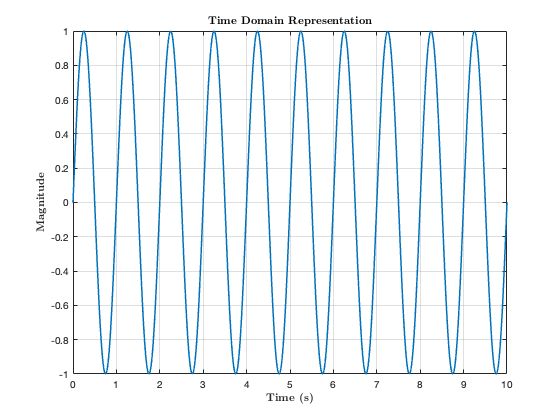
\includegraphics[scale=0.45]{IMAGES/Sine.png}
    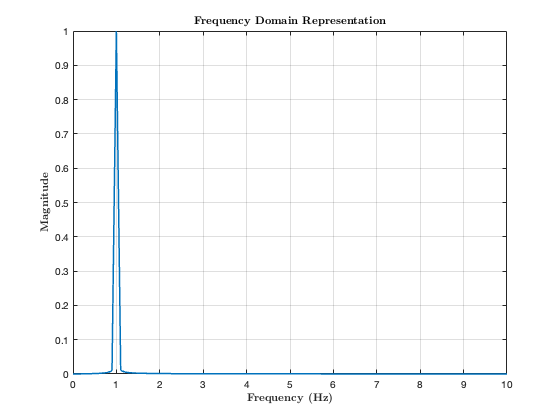
\includegraphics[scale=0.45]{IMAGES/Sine_FT.png}
    \caption{Time and Frequency Domain Representations of Sinusoid at $1Hz$}
    \label{fig:FT_example}
\end{figure}

The FT of the signal shows a peak at $1Hz$, which is the exact frequency of the signal present. However, in more real world examples, the FT of a signal can show multiple peaks at different frequencies as signals can have many different frequency components. In most cases, the FT is not directly computed, as it is quite inefficient to calculate as it takes $n^2$ operations. More commonly, a DSP algorithm called the Fast Fourier Transform (FFT) of a signal is calculated as it is far more computationally inexpensive, allowing for more complex signals to be analysed.

\subsection{Previous Work}
\textcolor{red}{Maybe change this name}

section plan:

\begin{itemize}
    \item talk about PYNQ and petalinux
    \item could talk about linux 
    \item important signal processing techniques
    \item Important communications fundamentals
    \item Digital Logic Design
    \item PL/PS design
    \item \textcolor{red}{Talk about AXI}
\end{itemize}

 
\newpage
\section{literature Review}

\begin{itemize}
    \item talk about different papers
    \item Where the idea originates from
    \item previous work completed
    \item Why does this work matter?  
    \item 
\end{itemize}

\newpage
\section{Project Methodology}
\subsection{Design Philosophy}
\begin{itemize}
    \item initial ideas and plans
    \item model composer design
    \item GNU Radio design
    \item Vivado design (IPI and code)
    \item 2x2 vs RFX design stages
    \item PYNQ and PetaLinux designs (would probably go in 2x2 and rfx sections respectively)
    \item PetaLinux - can talk about how to flash the image onto the card - different boot modes.
    \item time taken for design process
    \item iterative design process with small changes made to each design
    \item potentially recovering the card from different states
    \item Initial testing with RFX - spectrum analyser from BittWare
    \item With axi stream, talk about how the data needs to be formatted before being sent out.
    \item Talk about ILA t
    \item \textcolor{red}{talk about gnu radio proposed design}
    \item \textcolor{red}{talk about issues ran into that and why u made changes to fix them - then go into more detail in Discussion}
\end{itemize}                          
\newpage

The  system design featured a transmitter and receiver setup, linking the DAC and ADC via an SMA coaxial RF cable. This approach is commonly employed as an introductory step in SDR development, as it provides a strong foundation in radio architecture and the associated development cycle. The design was subsequently validated on both the BittWare RFX card and the RFSoC 2x2 development board. Multiple platforms were utilized to leverage the advantages of the 2x2 board’s simpler PS interface, PYNQ. PYNQ offers significantly more online documentation, theoretically enabling a faster and more efficient development process compared to PetaLinux. Unlike PetaLinux, where each image is tied to a specific hardware configuration, PYNQ’s overlays allow for greater flexibility, facilitating a more adaptable development workflow.
 
\subsection{Digital Logic Design}

Primarily, the digital logic was designed using Vitis Model Composer through MATLAB and Simulink. This software abstracts the need to extensively write VHDL code, which can be very tenuous and time consuming, by using a number of pre-defined \enquote{blocks}, ranging from simple adders, to more complex operations such as the Fourier Transform. The digital logic in this design will realise an AM transmitter ($T_X$) and receiver ($R_X$). A high level overview of this system can be seen below in Figure \ref{fig:am_tx_rx}.

\begin{figure}[h]
   \centering
    \begin{circuitikz}
        % TX side
        \draw (0, 0) node[mixer, fill=yellow!50](mix){Mixer};
        \draw (mix.w) -- ++(-1, 0) to[twoport, fill=red!50, t=$NCO$, l_=Data Step Size]  ++(-1, 0) -- ++(-1.5, 0);
        \draw (mix.e) -- ++(1, 0) -- ++(0, 1) node[dinantenna](ant1){} node[left]{$T_X$}
        \draw[thick] (ant1.s) -- ++(0, -1);
        \draw [latex-] (0,-0.5) -- ++(0,-2) node[midway, right] {};

        % TX Antenna Waves
        \draw[thick](ant1.right) node[waves, xscale=0.8, anchor=left](){};
        
        % RX side
        \draw (5, 0) node[mixer, fill=yellow!50](mix2){Mixer};
        \draw (mix2.w) -- ++(-1, 0) -- ++(0, 1) node[dinantenna](ant2){} node[right]{$R_X$};
        \draw[thick] (ant2.s) -- ++(0, -1);
        \draw (mix2.e) -- ++(1, 0) to[lowpass, fill=cyan!30, l=LP Filter] ++(1, 0) -- ++(1.5, 0);
        \draw [latex-] (5,-0.5) -- ++(0,-2) node[midway, right] {};

        % RX NCO
        \draw (0, -2.5) to[twoport, t=$NCO$, fill=red!50, l=Carrier Step Size] ++(5, 0);
        \draw [latex-] (2.5,-3) -- ++(0,-1.5) node[midway, right] {};

    \end{circuitikz}

    \caption{High Level Overview of AM Transmitter and Receiver System}
    \label{fig:am_tx_rx}
\end{figure}

\subsubsection{Transmitter Design}

\textcolor{red}{Mention about the designs using AXI}

The transmitter was designed as a \enquote{data generation} block, which is then sent to the RFDC. To verify the functionality of the design, the transmitter would generate a sine wave through a Numerically Controlled Oscillator (NCO). The NCO subsystem used in both the transmitter and receiver design is shown in Figure \ref{fig:nco figure}.

\begin{figure}[h]
    \centering
    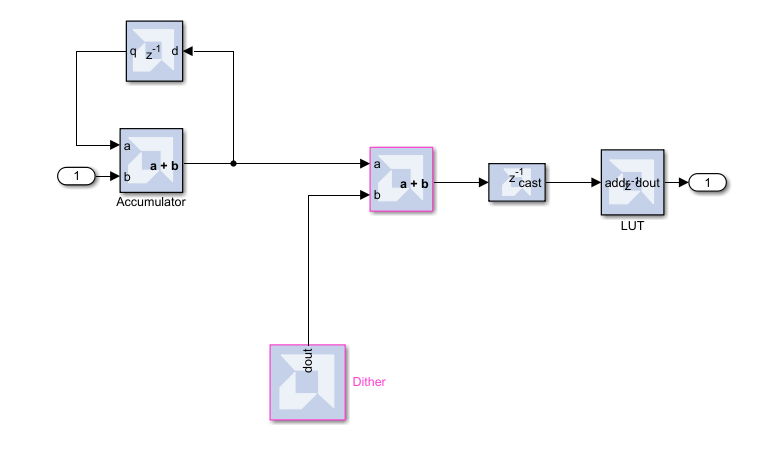
\includegraphics[scale=0.7]{IMAGES/NCO_model_composer.PNG}
    \caption{NCO in Vitis Model Composer}
    \label{fig:nco figure}
\end{figure}

NCOs are comprised of two main components, a Look Up Table (right), which is a form of Read Only Memory (ROM), along with an accumulator (left). The accumulator is implemented in Model Composer using two components, an adder and a delay. The adder counts up a certain rate, depending on the inputted step size due to the output being fed back to the input. For example, if the input to the accumulator was 1, then the accumulator would output all integer values from 0 up to the wordlength of the output data. The LUT stores, in this case, quantised values of a sinusoid, which are indexed by the output of the accumulator. Along with the two main components of this NCO, there is an extra block which adds \enquote{dithering} to the system. This is when a low level of noise is added to the system to improve its Spurious Free Dynamic Range (SFDR) \cite{nco_notes}, a common figure of merit for RF systems. SFDR is defined as the ratio of the strongest signal present to the largest spurious signal present \cite{SFDR_paper}.

As mentioned above, the input to an NCO is called the step size, which determines the set frequency that the NCO can output. Step size can be calculated using a number of defined system parameters through Equation \ref{eq:step size}.

\begin{equation}
    \mu = N\frac{f_d}{f_s}
    \label{eq:step size}
\end{equation}

Where $N$ is the depth of the LUT, $f_d$ is the desired output frequency of the NCO, and $f_s$ is the sampling frequency of the system. The accumulator of the NCO generates $n$ number of address bits which then determines the depth of the LUT through Equation \ref{eq:LUT depth}.

\begin{equation}
    N = 2^n
    \label{eq:LUT depth}
\end{equation}

The transmitter design features two NCOs, one which generates the data signal, and one for the carrier signal. Modulation, in this case, refers to carrier modulation, which is when a signal is multiplied by a carrier frequency to be transmitted across a channel. The other type of modulation is called baseband modulation, and refers to the transformation of digital bits to \enquote{symbols} in a communications system. The transmitter design in Model Composer can be seen below in Figure \ref{fig:transmitter design}.

%Need to get new photo for this - make components closer and remove that scope
\begin{figure}[h]
    \centering
    
\includegraphics[scale=0.6]{IMAGES/data_generator_model_composer.PNG}
    \caption{Transmitter Design in Vitis Model Composer}
    \label{fig:transmitter design}
\end{figure}

The first input to this design (\textit{tdata\_in}), seen at the top of Figure \ref{fig:transmitter design}, is streamed from the PS and selects the NCO frequency to output through a multiplexer (MUX). The second input is used to essentially turn the NCOs on and off. This is done through an enable pin that only allows the MUX to pass the step size input when the signal \textit{mux\_en} is set high (1). For simplicity at the receiver side, only one carrier frequency was used for both values of tdata\_in.


An amplitude modulated signal can be described as the product of a low frequency data signal, $D(t)$, and a carrier signal, $C(t)$. The notation for the data signal is shown in Equation \ref{eq:data signal}


\begin{equation}
    D(t) = Acos(2\pi f_dt) 
    \label{eq:data signal}
\end{equation}

With amplitude $A$, and frequency, $f_d$. Similarly, the carrier signal is defined as:

\begin{equation}
    C(t) = cos(2\pi f_ct)
    \label{eq: carrier signal}
\end{equation}

Following on from this, the modulated signal, $S(t)$, can then be derived using relatively simple trigonometry.

\begin{equation}
\begin{aligned}
   S(t) =  D(t)\times C(t) &= Acos(2\pi f_dt) cos(2\pi f_ct)\\
     &= \frac{A}{2} \left[cos(2\pi (f_c-f_d)t)+cos(2\pi (f_c+f_d)t)\right]
\end{aligned}
\end{equation}


\subsubsection{Receiver Design}

The Receiver is designed to essentially reverse the operations that the transmitter does to the signal. This means that the incoming signal is demodulated, and low pass filtered. The need for filtering after demodulation can be explained through some simple mathematics. To demodulate an AM signal, the incoming signal is multiplied again by the original carrier frequency.

\begin{equation}
\begin{aligned}
    Y(t) &= S(t)\times C(t)\\
    &= \frac{A}{2} cos(2\pi f_c t) \left[cos(2\pi (f_c-f_d)t)+cos(2\pi (f_c+f_d)t)\right]\\
    &= \frac{A}{2}cos(2\pi f_c t)cos(2\pi(f_c-f_d)t)+\frac{A}{2}cos(2\pi f_c t)cos(2\pi(f_c+f_d)t)\\
    &= \frac{A}{4}cos(2\pi(2f_c-f_d)t)+\frac{A}{4}cos(2\pi f_dt)+\frac{A}{4}cos(2\pi(2f_c+f_d)t)+\frac{A}{4}cos(2\pi f_dt)\\
    &= \frac{A}{2}cos(2\pi f_dt) + \frac{A}{4}\left[cos(2\pi(2f_c-f_d)t)+cos(2\pi(2f_c+f_d)t)\right]\\
    \label{eq:demodulation_maths}
\end{aligned}
\end{equation}

At the end of the demodulation stage, there are 2 components left in the signal, the original, baseband frequency component, and the left over modulated component at the carrier frequency. Therefore, a low pass filter can be implemented to remove any of the unwanted carrier signal left after demodulation. The model for the receiver in Model Composer can be seen below in Figure \ref{fig:receiver_model_composer}.

\begin{figure}[h]
    \centering
    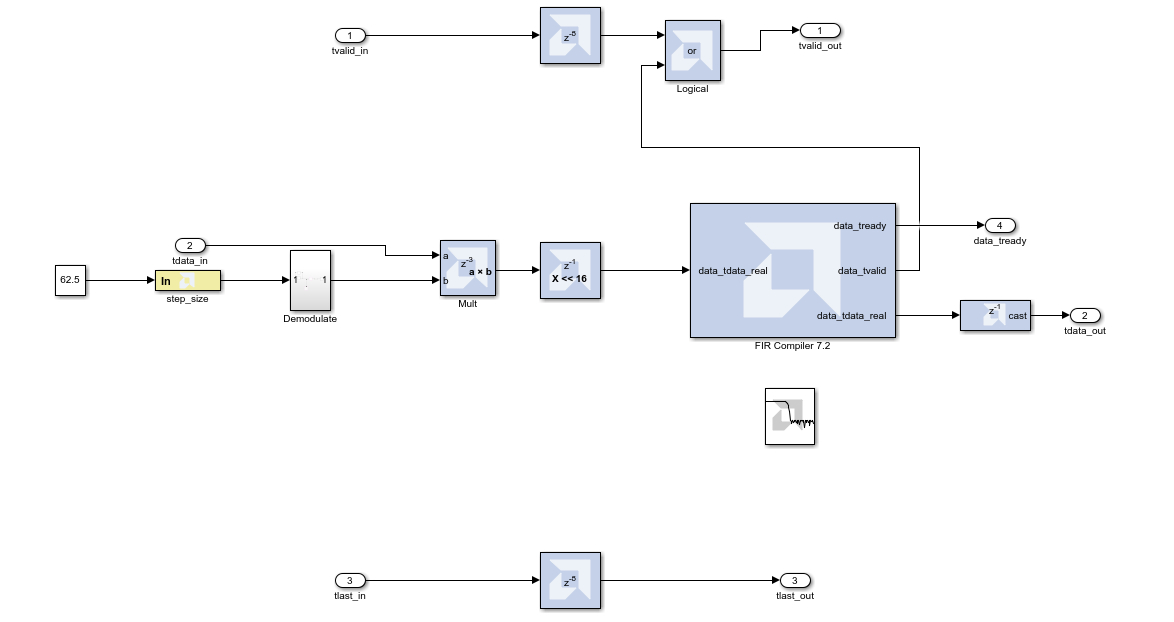
\includegraphics[scale=0.6]{IMAGES/Receiver_model_composer.PNG}
    \caption{Receiver Design in Vitis Model Composer}
    \label{fig:receiver_model_composer}
\end{figure}

The receiver takes the input of the RF-ADC and demodulates it with an NCO set to output the same carrier frequency as the transmitter. Following on from the initial demodulation stage is the filtering stage, which is comprised of a low pass Finite Impulse Response (FIR) filter, which was implemented into the FIR compiler block from Model Composer. The filter coefficients were designed using MATLABs \textbf{fir2()} function, which takes a number of arguments to specify the order, cut off frequency, and magnitude characteristics. The magnitude and phase response of this filter can be seen below in Figure \ref{fig:FIR response}.

\begin{figure}[h]
    \centering
    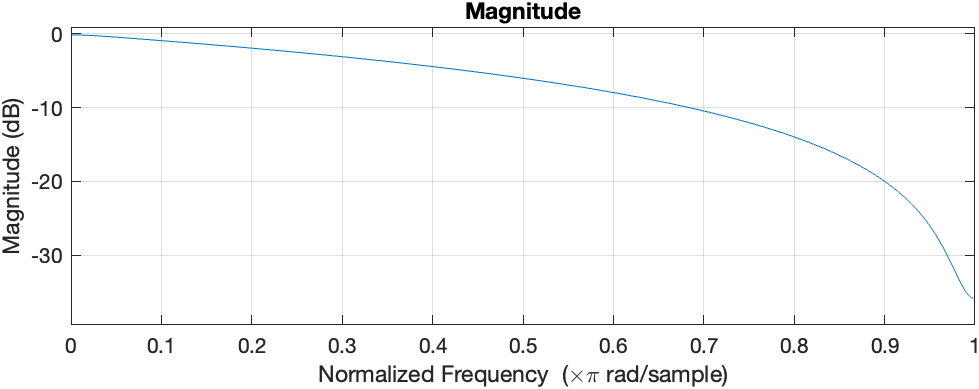
\includegraphics[scale=0.8]{IMAGES/untitled1.png}\\
    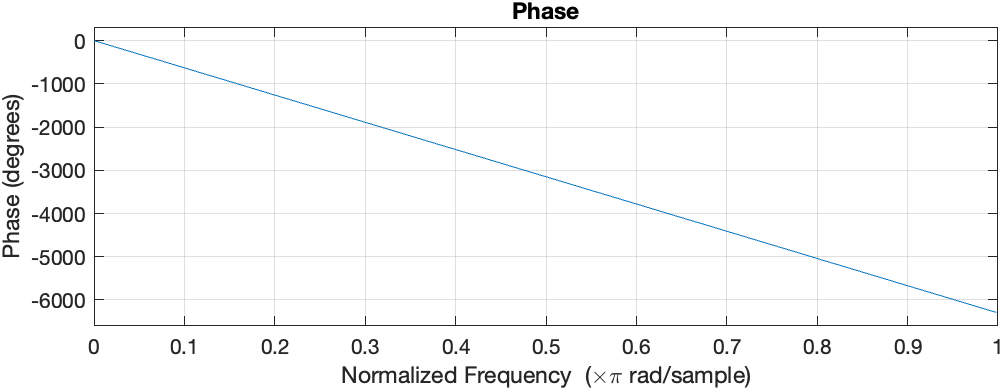
\includegraphics[scale=0.8]{IMAGES/untitled2.png}
    \caption{Magnitude and Phase Response of Low Pass FIR Filter}
    \label{fig:FIR response}
\end{figure}

\subsubsection{IP Integrator Design}

Model Composer is a great tool for testing the functionality of a hardware design through simulations, but to actually implement the designs, HDL code must be generated using the system generator tool. This tool allows a user to specify the target hardware device (or chip) and generate custom code, either in VHDL or Verilog to then be exported as IP, to then be used in Vivado's IP Integrator (IPI) tool. Since Vivado projects are specific to the target hardware, separate projects for the RFSoC 2x2 and the RFX were needed, due to the difference in both chip generations and design goals.

\paragraph{RFSoC 2x2 Design Validation} 

Given the lack of accessibility of the RFX, it was decided that the best approach for testing and developing this project was to use the RFSoC 2x2 development board as a means to work on the project whilst unable to visit the BittWare office. The 2x2 was used to verify the functionality of the transmitter and receiver designs from Model Composer on real hardware through a loopback configuration. Custom IP generated from Model Composer can be added by pointing to the \enquote{ip} folder (found inside the \enquote{netlist} folder of the Model Composer project) in Vivado. After IP is added, it can be used in any block design and connected to a number of proprietary IP blocks that come standard with Vivado. Figure \ref{fig:2x2_IPI} shows the Loopback configuration model on the RFSoC 2x2 in Vivado's IP integrator.

\textcolor{red}{maybe look a changing photo to more vertical to get better fit}

\begin{figure}[h]
    \centering
    
\includegraphics[scale=0.5]{IMAGES/2x2_IPI.PNG}
    \caption{Vivado IP Integrator Design for RFSoC 2x2 Loopback Configuration}
    \label{fig:2x2_IPI}
\end{figure}

To read from the output of the receiver, and write to the input of the transmitter, an AXI Direct Memory Access (DMA) controller was used. The AXI DMA is instructed by a processor core, in this case the PS, to move data between points in a design \cite{strathsdr_axi}. The DMA is used for accessing the shared memory between the PS and PL, allowing for high speed data transfers between different IP. At the core of this design is the ZYNQ Ultrascale+ RF Data Converter, which is the equivalent IP core of the RFDCs previously mentioned. The RFDC IP core combines the RF-ADC and RF-DAC in one single package, with  data being inputted to the DAC side, and received from the ADC side.

Configuring the RFDCs in Vivado takes significant design effort, as the master and slave sides can potentially require different clocking speeds, which complicates design efforts as the correct clock has to be meticulously connected to each component on both the transmit and receive side. It is best practice to clock everything on the transmit side with the same frequency as the RF-DAC, and do the same for the receive side with the RF-ADC. Doing so limits the risk of crossing a clock domain, which can make the design fail timing requirements (an important metric in FPGA programming) and have a plethora of issues in practice. A clock domain is a region of the FPGA that operates from a single clock source \cite{ClockDomainCrossing}. In this design, there are three clock domains, one for the transmit side, one for the receive side, and another for the PL. The RFDCs have a built in mixer, for doing further modulation up to extremely high frequencies, to transmit 5G signals, for example. However, this mixer was not used, this was to demonstrate the signal generated in hardware, along with the custom mixer that modulates and demodulates the signal. After the RFDCs were configured, the ADC and DAC output clocks were then connected to their respective parts of the design for transmitting and receiving. The RF-ADC could only output a $64MHz$ output clock, which is significantly slower than the required $128MHz$. To solve this issue, a \textbf{Clocking Wizard} IP was used to increase the clock frequency to its required value.

\textcolor{red}{clocking settings?}

Notice that there are two \enquote{sub-blocks} within this design, with one for the transmit side, and another for the receive side. This has been done to mitigate the crossing of clock domains inside of the hardware design. Figure \ref{fig:TX_sub-block} shows the transmit side sub-block.

\begin{figure}[h!]
    \centering
    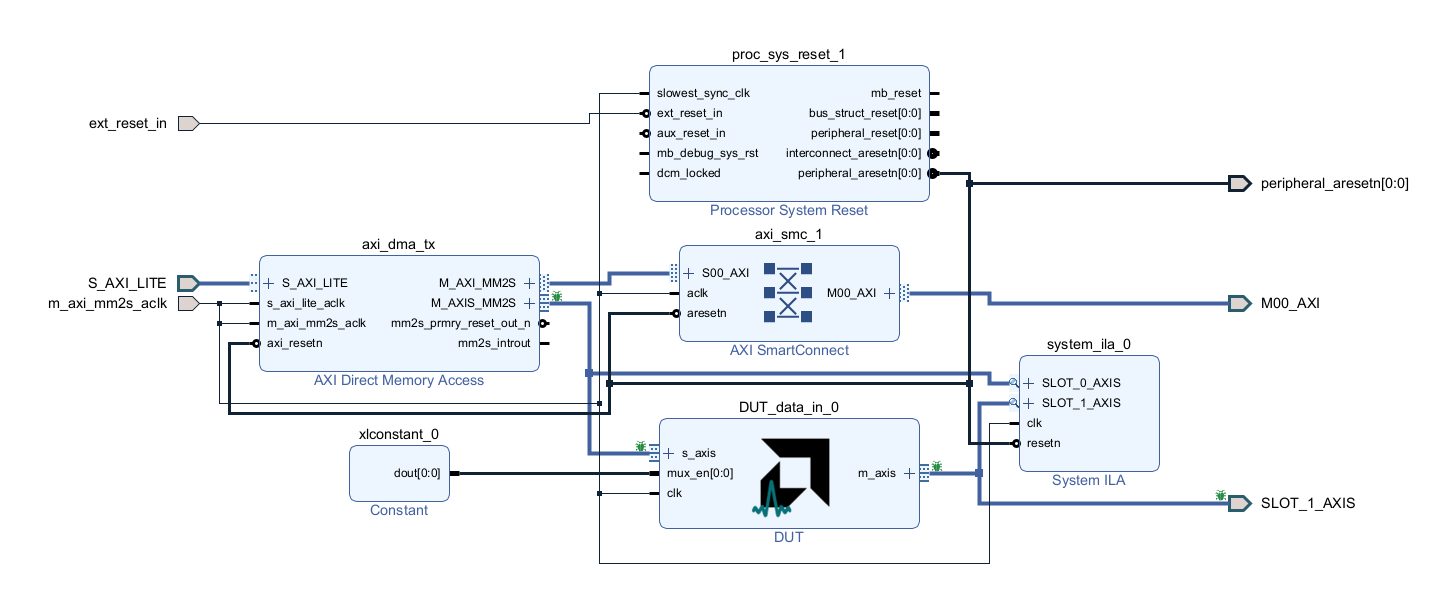
\includegraphics[scale=0.45]{IMAGES/TX_IPI.PNG}
    \caption{Transmit Side Sub-Block Inside Vivado IP Integrator}
    \label{fig:TX_sub-block}
\end{figure}

It must be noted that there is now 2 DMA IP cores within this design, one specifically for reading, and another for writing. In practice, this would operate by sending a DMA buffer (a certain amount of allocated memory for the DMA IP to access through read and write channels on the PS) to the custom transmit IP, which then starts the NCO to send a signal. In the software, the DMA buffer would then be read from the output of the receive side DMA, confirming the loopback configuration. The two sub-blocks were created to completely separate both the ADC and DAC clocks, therefore reducing any problems that can occur when crossing clock domains.

The RFSoC 2x2 is no longer manufactured and has since been replaced by the newer RFSoC 4x2, this means that using newer versions of Vivado can be difficult since the board files are not included with the Vivado package. The board files can be independently used in Vivado through some Tcl commands that can be found on the RFSoC website.

\paragraph{BittWare RFX-8440 2x100gbe Design Implementation} The Design implementation for the RFX is slightly different to that of the RFSoC 2x2, as the custom transmitter and receiver were instantiated as components inside of a significantly larger design. When shipping their cards, BittWare includes a number of \enquote{reference} designs, which are used to help customers understand and test the operation of the card, without having to design systems completely from the ground up. This design approach was taken for this project, as the previously mentioned transmitter and receiver were implemented within a larger design, rather than a fully custom one. The reference design in this case is the RFX8440-2x100gbe, which configures the entire FPGA, including all RFDC channels, the gigabit transceivers, and the PS. The project is aptly named because of it uses the two 100 gigabit Ethernet Quad Small Form-factor Pluggable (QSFP) transceivers, which can be connected to the card for high speed optical communications. The block diagram from BittWare's framework logic guide of the 2x100gbe design can be seen in Figure \ref{fig:2x100gbe_block_diagram} \cite{RFX_framework}.

\textcolor{red}{TALK ABOUT THE FOLDER STRUCTURE}

\begin{figure}[h!]
    \centering
    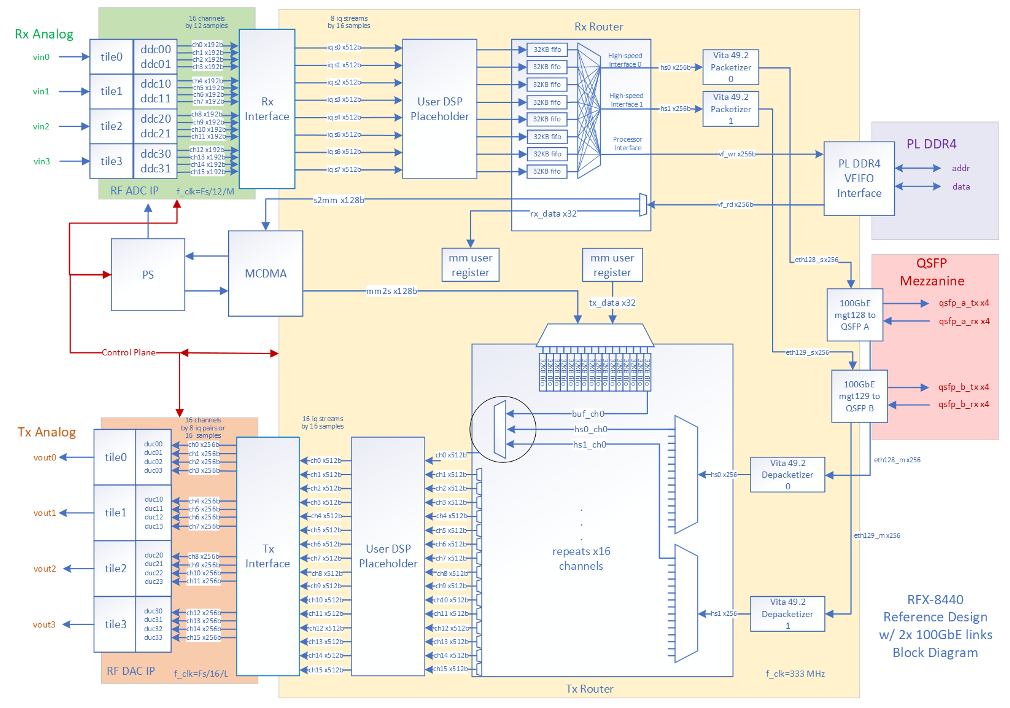
\includegraphics[scale=1]{IMAGES/Picture 1.png}
    \caption{Block Diagram of BittWare RFX-8440 With 2x100GBE Links}
    \label{fig:2x100gbe_block_diagram}
\end{figure}

This design is highly complex, since it features all components of the FPGA in a single bitstream. Inside of the design, and in Figure \ref{fig:2x100gbe_block_diagram}, is the DSP placeholder block, which has been designed for customers or other engineers to implement there own form of DSP without having to reconfigure the entire design with all of the I/O. Despite what Figure \ref{fig:2x100gbe_block_diagram} shows, the DSP placeholder is not an actual block inside of the Vivado IP integrator design that can be replaced with the users IP, but rather a VHDL file named \textbf{ii\_dsp\_top.vhd}. Functionally, this file connects the RFDCs together, involving no DSP at either the DAC or ADC side. The reference designs are inside a folder that can be downloaded or purchased by customers that may be interested in starting their designs from a known point. Building the Vivado project involves navigating to the 2x100gbe project folder inside of the Vivado Tool command language (Tcl) console \cite{AMD_Vivado_Tcl}, then running the \textbf{Build\_Vivado.tcl} script. This script launches the project and builds the block design(s) with the necessary IP added, and connections already made, a process which can take up to an hour.

Implementing custom IP inside of the 2x100gbe design is slightly different to that of the 2x2 design, as it is not added inside of a block design, but rather through a component instantiation using VHDL. When the transmitter IP is added to the project, its output products are generated, which includes an instantiation template inside of the \textbf{.vho} file. VHDL components are how separate top level entity declarations can be re-used inside of other designs. The component definition for the transmitter design can be seen in Listing \ref{list: tx def}.

\begin{listing}[h!]
\begin{minted}{vhdl}
COMPONENT DUT_data_in_16bit
  PORT (
    s_axis_tvalid : IN STD_LOGIC_VECTOR(0 DOWNTO 0);
    s_axis_tdata  : IN STD_LOGIC_VECTOR(0 DOWNTO 0);
    s_axis_tlast  : IN STD_LOGIC_VECTOR(0 DOWNTO 0);
    m_axis_tready : IN STD_LOGIC_VECTOR(0 DOWNTO 0);
    mux_en        : IN STD_LOGIC_VECTOR(0 DOWNTO 0);
    clk           : IN STD_LOGIC;
    m_axis_tvalid : OUT STD_LOGIC_VECTOR(0 DOWNTO 0);
    m_axis_tdata  : OUT STD_LOGIC_VECTOR(15 DOWNTO 0);
    m_axis_tlast  : OUT STD_LOGIC_VECTOR(0 DOWNTO 0);
    s_axis_tready : OUT STD_LOGIC_VECTOR(0 DOWNTO 0)
  );
END COMPONENT;

\end{minted}
\caption{Transmitter Component Definition}
\label{list: tx def}
\end{listing}

After defining the component inside of the \textbf{dsp\_top} entity, it can then be instantiated, as in Listing \ref{list: component instantiation}.

\begin{listing}[h!]
\begin{minted}{vhdl}
  fraser_user_code : DUT_data_in_16bit
  PORT MAP (
    s_axis_tvalid => "1",
    s_axis_tdata => nco_driver,
    s_axis_tlast => "1",
    m_axis_tready => m_axis_tx_tready(0 downto 0),
    mux_en => nco_mux_en,
    clk => axis_clk,
    m_axis_tvalid => m_axis_tx_tvalid(0 downto 0),
    m_axis_tdata => m_axis_tdata_temp,
    m_axis_tlast => m_axis_tx_tlast(0 downto 0),
    s_axis_tready => open
  );
\end{minted}
\caption{VHDL Transmitter Component Instantiation}
\label{list: component instantiation}
\end{listing}

The component instantiation is what actually includes the component in the design, where the signals from the 2x100gbe design are connected to the inputs and outputs of the custom transmitter. The 2x100gbe design configures all of the RF-ADC and RF-DAC channels, however, the goal is to only transmit over one channel, which means the transmitter component needs to take over one of these channels. The transmitter component 
\textcolor{red}{need to finish this section - get code from bittware and images}



\newpage
\subsection{Processing System Design}

Although the design of the PL is crucial to the physical operation of the FPGA, the PS design is crucial in interfacing and monitoring SoC devices through different development kits such as PYNQ and PetaLinux.

\subsubsection{PYNQ}

Starting with the PYNQ design for the RFSoC 2x2, this is created through a jupyter notebook interfacing with different Python libraries. After building the project for the 2x2 and generating the bitstream, the block design was then exported to the default file locations. To obtain the overlay, a shell script was written to save time navigating through the file system trying to find the \textbf{.bit} and \textbf{.hwh} files. The script also saves the overlays into the \textbf{Overlays} folder whilst keeping a copy of the files in their normal location. The names of the two files must be the same otherwise PYNQ will not recognise the overlay, the script also takes care of this.

After loading the overlay into the board, the IP contents of the bitstream can be inspected using the two lines of code found in Listing \ref{list:overlay_content}.

\begin{listing}[H]
\begin{minted}{vhdl}
ol = Overlay("Design_1_wrapper.bit")
ol? 
\end{minted}
\caption{Python Code for Inspecting Overlay Content}
\label{list:overlay_content}
\end{listing}

The question mark operator exports the contents of the bitstream into the jupyter notebook environment to ensure the right overlay is being used. From there, the controllable IP cores can be assigned to a Python variable, which allows for more readable code when calling different functions inside of the notebook.

After loading the overlay onto the FPGA, it is necessary to configure the reference clocks in software before initiating any PS–PL communication. The two required reference clocks for configuring the 2x2 board are the LMX and LMK clocks. These reference clocks are aptly named because they provide a high precision, low jitter clock for the RFDCs to use as a reference when generating their own clocks. Jitter refers to the variation in clock period between two consecutive cycles over a span of 1000 cycles \cite{jitter}. The required frequencies for the LMK and LMX clocks can be found in the  Xilinx PYNQ GitHub repository, specifically in the \textbf{xrfclk} package, which also includes a built in function to set the reference clocks with user defined frequencies, according to the board.

Although the RFDCs are pre-configured in hardware, they must also be properly initialized in software for the design to function correctly. Extensive resources are available online for configuring RFDCs, with the StrathSDR GitHub page being a particularly valuable source, offering numerous open-source projects that utilize RFSoC and configure it through PYNQ. This is achieved using the \textbf{xrfdc} Python package, which provides an interface to the RFDCs, ensuring proper clock configuration, dynamic Phase-Locked Loop (PLL) adjustments without requiring a bitstream reload, and setting mixer parameters along with Nyquist zones. The data converter settings are configured in two Python function declarations, but can be altered by the user to specify different sampling frequencies, or ADC/DAC tiles. The settings for the RFDCs have the mixer configured as a fine mixer that outputs $0Hz$ to allow for correct DAC and ADC mixing. Even though no mixer was used in the hardware configuration, the older generation RFSoCs expect some mixer settings to be applied in software to allow for correct configuration so this was chosen since it would not interfere with the incoming signal and still allow for data transmission.

Following on from this, the PS-PL communication could be established. This was done through the assignment of the both the DMAs and RFDC to a Python variable, which could be called back later when transferring data. The exact name of the IP that is assigned to the variable can be found through the previously mentioned $(?)$ operator under the \textbf{IP Blocks} section. The variable is then assigned through the use of the $(.)$ operator to assign a new variable to specific IP. Listing \ref{list:DMA Assignment} shows the assignment of a variable $tx\_dma$ to the transmit side DMA block.

\begin{listing}[h]
\begin{minted}{vhdl}
tx_dma = ol.TX.axi_dma_tx
\end{minted}
\caption{Python DMA Variable Assignment}
\label{list:DMA Assignment}
\end{listing}

Finally, the built-in \textbf{Allocate} package is used to allocate DMA buffers in memory which can then be transferred between PS and PL. In this design, both the send buffer and the receive buffer both have a size of 4000 samples (the maximum at which PYNQ allows), to ensure clarity when receiving data. The data can then be sent using the \textbf{transfer} function on both the send and receive DMA channels. These lines of code are then followed by the \textbf{wait} function which waits until the DMA channel goes back to an idle state. Following on from this, the received DMA buffer can be plotted using the \textbf{matplotlib} package, a comprehensive tool for data visualisation and plotting.

\subsubsection{PetaLinux}

PetaLinux has a more complex deployment process, as a PetaLinux image needs to be accompanied by a specific bitstream. This means that testing and confirming design choices can take significantly longer when working with a board that does not support PYNQ. BittWare thankfully has a set build process for creating and customising PetaLinux images through some documentation and build scripts. However, the RFX needs specific hardware settings to configure properly, specifically on the PS, which needs to have a number of different ports enabled for communication with the images boot file system. This means that creating completely custom images in PetaLinux can be a painstaking and long process which takes significant design effort and time. This is another reason as to why the reference design was used, as the hardware design was properly configured to allow the PetaLinux image to build and run properly, as it had been through significant testing throughout its design stage.

The first step in creating the PetaLinux image is to export the hardware image (bitstream) to a \textbf{.xsa} file, saved in the specified PetaLinux folder within the larger reference design folder. This xsa file is slightly different to the overlays seen in PYNQ development, as it features a number of different files inside which tell the PetaLinux build about the hardware design - rather than the two overlay files that PYNQ needs to configure hardware. Although, newer PYNQ releases do feature support for xsa files, which streamlines the development process slightly, since the \textbf{.bit} and \textbf{.hwh} files do not need to be found within the file structure of the Vivado project.


\newpage
\section{Results and Analysis}

\begin{itemize}
    \item testing of 2x2 and results, how this differs from RFX  
    \item Initial testing with RFX - spectrum analyser from BittWare
    \item All resulting graphs and waveforms - troubles of different sections
    \item Talk about ILA for debugging on RFX
    \item Talk about adding the constant lmk\_reset.
    \item 
\end{itemize}


\begin{figure}
    \centering
    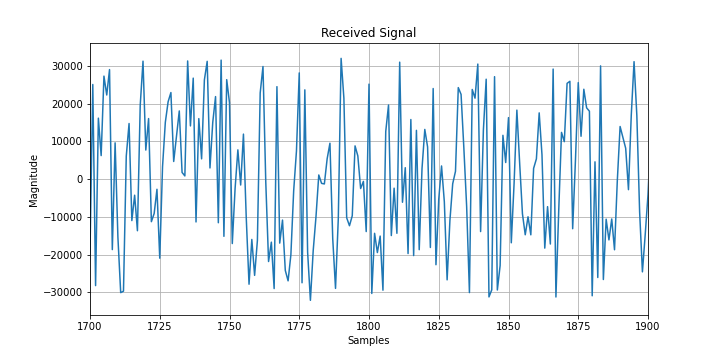
\includegraphics[scale=0.7]{IMAGES/received_zoomed.png}
    \caption{Caption}
    \label{fig:enter-label}
\end{figure}


\newpage
\section{Conclusion and Further Work}
\newpage
\bibliographystyle{ieeetr}
\bibliography{citation}
\end{document}
